%%% ACM Transactions on Software Engineering and Methodology (TOSEM)
%%% Structural Fuzzing: Adapting Input Mutation Testing for Parameterized Model Validation
%%% Anonymous review submission

\documentclass[manuscript,review,anonymous]{acmart}

%% Packages
\usepackage{algorithm}
\usepackage{algorithmic}
\renewcommand{\algorithmiccomment}[1]{\hfill$\triangleright$ \textit{#1}}
\usepackage{booktabs}
\usepackage{multirow}
\usepackage{xcolor}
\usepackage{pgfplots}
\pgfplotsset{compat=1.18}
\usepgfplotslibrary{statistics}

%% Custom commands
\newcommand{\MAE}{\mathrm{MAE}}
\newcommand{\MRI}{\mathrm{MRI}}
\newcommand{\BI}{\mathrm{BI}}

%% Journal and copyright metadata
\acmJournal{TOSEM}
\setcopyright{none}           % Appropriate for anonymous review submission
\acmDOI{}                     % Will be assigned by ACM
\acmYear{2026}
\acmVolume{0}
\acmNumber{0}
\acmArticle{0}

%% ============================================================
%% CCS Concepts
%% ============================================================
\begin{CCSXML}
<ccs2012>
   <concept>
       <concept_id>10011007.10011074.10011099</concept_id>
       <concept_desc>Software and its engineering~Software testing and debugging</concept_desc>
       <concept_significance>500</concept_significance>
   </concept>
   <concept>
       <concept_id>10011007.10011074.10011092</concept_id>
       <concept_desc>Software and its engineering~Search-based software engineering</concept_desc>
       <concept_significance>500</concept_significance>
   </concept>
   <concept>
       <concept_id>10010147.10010257.10010293</concept_id>
       <concept_desc>Computing methodologies~Model verification and validation</concept_desc>
       <concept_significance>500</concept_significance>
   </concept>
</ccs2012>
\end{CCSXML}

\ccsdesc[500]{Software and its engineering~Software testing and debugging}
\ccsdesc[500]{Software and its engineering~Search-based software engineering}
\ccsdesc[500]{Computing methodologies~Model verification and validation}

\keywords{fuzzing, mutation testing, model validation, robustness testing, sensitivity analysis, structural testing, parameter mutation, Model Robustness Index}

%% ============================================================
%% Title and Author
%% ============================================================
\title{Structural Fuzzing: Adapting Input Mutation Testing for Parameterized Model Validation}

\author{Andrew H. Bond}
\email{andrew.bond@sjsu.edu}
\orcid{0009-0003-2599-6158}
\affiliation{%
  \institution{San Jos\'{e} State University}
  \department{Department of Computer Engineering}
  \city{San Jos\'{e}}
  \state{California}
  \country{USA}
}

%% ============================================================
\begin{document}

\begin{abstract}
Software fuzzing---the automated generation of mutated inputs to discover program crashes---is a cornerstone of modern software testing.
Tools such as AFL and LibFuzzer mutate program \emph{inputs} (byte sequences) and monitor for assertion failures, guided by code-coverage metrics.
We observe that parameterized predictive models face an analogous validation challenge: standard techniques (cross-validation, information criteria, Bayesian model comparison) test whether a model \emph{fits} data but not whether its structure is \emph{necessary}, \emph{sufficient}, or \emph{robust} under parameter perturbation.

We introduce \emph{structural fuzzing}, a six-component validation framework that adapts the adversarial mindset of software fuzzing to model validation by mutating structural \emph{parameters} rather than program inputs.
The six components are:
(1)~\emph{dimension enumeration}---exhaustive search over parameter subsets to find minimal sufficient structure;
(2)~\emph{Pareto frontier extraction}---identifying models optimal at each complexity level;
(3)~\emph{sensitivity profiling}---ablation to rank parameters by predictive contribution;
(4)~the \emph{Model Robustness Index} (MRI)---a weighted-percentile robustness metric adapted from the Bond Index for LLM evaluator robustness;
(5)~\emph{adversarial threshold search}---systematic log-spaced search for the minimal perturbation that flips a prediction; and
(6)~\emph{compositional testing}---greedy parameter addition to reveal optimal ordering and diminishing returns.

We demonstrate the framework on a nine-dimensional geometric economics model predicting 16 behavioral targets across game theory, prospect theory, and published meta-analyses.
The campaign reveals that a three-dimensional subset achieves $\MAE = 2.70\%$ with all 16 targets passing within tolerance, that the monetary dimension has zero sensitivity, and that the model achieves $\MRI = 1.39$.
All structural parameters are discovered by automated search, not hand-tuned.
We further validate on a software defect prediction model, where the framework discovers that complexity and process metrics suffice while traditional size metrics (LOC) contribute minimally---consistent with decades of empirical SE findings.
The methodology is domain-general and applicable to any parameterized predictive model, including machine learning models, agent-based simulations, and scientific computing pipelines.
\end{abstract}

\maketitle

%% ============================================================
\section{Introduction}
\label{sec:intro}
%% ============================================================

Software fuzzing has transformed how practitioners discover latent defects.
Since Miller, Fredriksen, and So~\cite{miller1990} demonstrated that random byte sequences could crash 25--33\% of standard Unix utilities, the adversarial testing paradigm has matured into an indispensable pillar of the software engineering toolkit.
Coverage-guided fuzzers such as AFL~\cite{zalewski2014} instrument programs to track code-path coverage and preferentially mutate inputs that explore new branches.
Generation-based fuzzers such as LibFuzzer~\cite{serebryany2016} and Peach~\cite{eddington2009} leverage input grammars to produce structurally valid but semantically adversarial test cases.
The central principle is adversarial automation: \emph{do not ask whether the system works on the inputs you expect; ask what inputs break it}.
Manes et al.~\cite{manes2021} survey the field comprehensively, documenting hundreds of critical vulnerabilities discovered by fuzzing that conventional testing missed.

Parameterized predictive models---in science, engineering, and machine learning---face a structurally analogous validation challenge.
A model may pass cross-validation~\cite{stone1974}, achieve a low Bayesian Information Criterion (BIC)~\cite{schwarz1978}, and earn a favorable Bayes factor~\cite{kass1995}, yet depend on a fragile parameter configuration where a small perturbation changes predictions qualitatively.
Cross-validation tests whether the model generalizes to held-out \emph{data}, but it does not test whether the model's \emph{structure} is necessary, sufficient, or robust.
Information criteria penalize the \emph{count} of free parameters but treat all parameters as interchangeable---they cannot identify which structural components are load-bearing and which are redundant.
Bayesian model comparison is principled but computationally expensive, prior-dependent, and silent on adversarial robustness.

The replication crisis in psychology and economics~\cite{ioannidis2005,open2015} has made this structural fragility a pressing concern.
Simmons, Nelson, and Simonsohn~\cite{simmons2011} documented how ``researcher degrees of freedom''---undisclosed analytical flexibility in model specification and parameter selection---enable researchers to obtain statistically significant results from noise.
A model validation methodology that systematically probes structural robustness, rather than merely confirming predictive accuracy, would address a root cause of non-replicable findings.

This paper introduces \emph{structural fuzzing}: a systematic, six-component validation framework that adapts the adversarial mindset of software fuzzing from program inputs to model parameters.
Where software fuzzing mutates input bytes to find crashes, structural fuzzing mutates structural parameters to find prediction failures.
The analogy is precise:

\begin{itemize}
    \item The \emph{program under test} becomes the \emph{parameterized model}.
    \item The \emph{input bytes} become the \emph{structural parameters} (e.g., variance weights $\sigma^2$).
    \item A \emph{crash or assertion failure} becomes a \emph{prediction failure} (exceeding the error tolerance for an empirical target).
    \item The \emph{code-coverage metric} becomes the \emph{prediction target coverage} (fraction of empirical targets matched within tolerance).
    \item \emph{Coverage-guided mutation} becomes \emph{grid/random search} over parameter space.
    \item \emph{Crash minimization} becomes identification of \emph{minimal sufficient structure} via the Pareto frontier.
\end{itemize}

The six components of the framework are: (1)~\emph{dimension enumeration}, which performs exhaustive search over parameter subsets to find minimal sufficient structure; (2)~\emph{Pareto frontier extraction}, which identifies models optimal at each complexity level; (3)~\emph{sensitivity profiling}, which uses ablation to rank each parameter's contribution; (4)~the \emph{Model Robustness Index} (MRI), a scalar robustness metric adapted from the Bond Index~\cite{bond2026} for LLM evaluator robustness; (5)~\emph{adversarial threshold search}, which finds the minimal perturbation that flips a prediction; and (6)~\emph{compositional testing}, which builds the model parameter by parameter to reveal optimal ordering and diminishing returns.

We demonstrate structural fuzzing on two case studies.
First, a nine-dimensional geometric economics model~\cite{bond2026b} that predicts 16 behavioral targets spanning game theory, prospect theory, and published meta-analyses.
The campaign reveals that a three-dimensional subset (Social Impact, Virtue/Identity, Epistemic) achieves $\MAE = 2.70\%$ with 16/16 targets passing, that the monetary dimension contributes zero predictive value, and that the model achieves $\MRI = 1.39$.
Second, a software defect prediction model, where the framework automatically recovers the empirically established finding that complexity and process metrics dominate traditional size metrics~\cite{menzies2007,hall2012}.
Critically, all parameters are discovered by automated search---the structural findings are properties of the model and data, not artifacts of hand-tuning.

A note on terminology is warranted.
Structural fuzzing is best understood as a \emph{structural mutation-testing campaign inspired by fuzzing}.
It draws its adversarial mindset and systematic exploration strategy from software fuzzing, while its search mechanisms (grid search, random search, ablation) are closer to mutation testing and search-based software engineering.
The term ``fuzzing'' reflects two specific technical parallels beyond philosophy:
(1)~the adversarial threshold search (Algorithm~\ref{alg:adversarial}) performs binary search over perturbation intensity to find minimal failure-inducing mutations, directly analogous to AFL's crash minimization;
(2)~the MRI computation (Algorithm~\ref{alg:mri}) incorporates a \emph{feedback-guided refinement} phase: after an initial undirected perturbation round, perturbation directions that produced the largest deviations are preferentially resampled in a focused second round, analogous to AFL's strategy of retaining and further mutating inputs that discover new code paths.
This feedback loop ensures that the MRI reflects worst-case behavior in structurally vulnerable regions of parameter space, not merely average-case behavior over uniform random perturbations.

The paper is organized as follows.
Section~\ref{sec:background} reviews software fuzzing, ML model testing, the Bond Index, and existing model validation techniques.
Section~\ref{sec:framework} presents the six-component framework with algorithmic pseudocode.
Section~\ref{sec:implementation} describes the implementation and computational cost.
Section~\ref{sec:case_study} demonstrates the framework on two case studies: a geometric economics model and a software defect prediction model.
Section~\ref{sec:discussion} discusses generalizability, comparisons, and threats to validity.
Section~\ref{sec:conclusion} concludes.

%% ============================================================
\section{Background and Related Work}
\label{sec:background}
%% ============================================================

\subsection{Software Fuzzing}

Fuzzing---automated generation of random, mutated, or adversarial inputs to discover program defects---was introduced by Miller, Fredriksen, and So~\cite{miller1990}, who found that random byte sequences crashed 25--33\% of standard Unix utilities.
The technique has since evolved into two principal paradigms.

\emph{Mutation-based fuzzing}, exemplified by AFL (American Fuzzy Lop)~\cite{zalewski2014}, starts with valid seed inputs and applies random mutations: bit flips, byte insertions, arithmetic adjustments, and dictionary-based substitutions.
AFL's key innovation is \emph{coverage-guided feedback}: it instruments the program under test to track which code paths (basic-block transitions) are exercised by each input, and preferentially retains and further mutates inputs that exercise new paths.
This coverage guidance makes AFL vastly more effective than purely random fuzzing at reaching deep program states, because it directs the search toward unexplored regions of the program's behavior.

\emph{Generation-based fuzzing}, exemplified by LibFuzzer~\cite{serebryany2016} and Peach~\cite{eddington2009}, uses knowledge of the input format---a grammar, protocol specification, or API contract---to generate inputs that are structurally valid but semantically adversarial.
LibFuzzer integrates with the LLVM compiler infrastructure to provide in-process, coverage-guided fuzzing with low overhead, enabling billions of test executions per campaign.

Takanen, DeMott, and Miller~\cite{takanen2008} provide a comprehensive treatment of fuzzing methodologies for software security testing.
Manes et al.~\cite{manes2021} survey the field, cataloging fuzzing techniques along five dimensions: the source of test cases (mutation vs.\ generation), the feedback mechanism (coverage vs.\ none), the target granularity (function, program, protocol), the oracle (crash, sanitizer, differential), and the search strategy (random, evolutionary, gradient-based).

Three properties of software fuzzing motivate structural fuzzing for model validation:

\begin{enumerate}
    \item \textbf{Adversarial framing.} The goal is to find failures, not to confirm correctness. The methodology is designed to discover fragility.
    \item \textbf{Exhaustiveness within budget.} Fuzzing explores the input space as thoroughly as the computational budget allows, rather than testing a fixed set of hand-selected cases.
    \item \textbf{Minimal failure identification.} When a failure is found, fuzzing tools minimize the failing input to isolate the root cause. AFL's crash minimization reduces a crashing input to the smallest input that still triggers the same crash.
\end{enumerate}

\subsection{Machine Learning Model Testing}

The software engineering community has increasingly applied testing concepts to machine learning models.
Pei et al.~\cite{pei2017} introduced DeepXplore, which adapts neuron coverage (analogous to code coverage) to generate inputs that maximize the number of activated neurons in deep neural networks, discovering thousands of erroneous behaviors in production DNN models.
This work established the principle that coverage-guided input generation---the core idea of software fuzzing---transfers effectively to ML model testing.

Metamorphic testing~\cite{segura2016} addresses the oracle problem in ML testing: when the expected output for a given input is unknown, metamorphic relations (e.g., ``rotating an image should not change its classification'') provide implicit specifications that can be checked automatically.
Segura et al.~\cite{segura2016} survey metamorphic testing applications across search engines, compilers, machine learning systems, and scientific software.

Property-based testing, popularized by QuickCheck in the functional programming community, generates random inputs constrained by user-specified properties and searches for counterexamples.
The structural fuzzing framework shares the property-based testing philosophy: the ``properties'' are the prediction targets (empirical observations that the model should match within tolerance), and the ``random inputs'' are the structural parameters.

Our work differs from these approaches in a fundamental respect: we mutate the model's \emph{structural parameters} rather than its \emph{inputs}.
DeepXplore and metamorphic testing ask ``what inputs cause the model to fail?''---a question about the model's input-output behavior.
Structural fuzzing asks ``what parameter configurations cause the model to fail?''---a question about the model's structural robustness.
This distinction is analogous to the difference between testing a bridge with heavy loads (input testing) and testing whether the bridge collapses if a support beam is weakened (structural testing).

\subsection{The Bond Index}

The Bond Index~\cite{bond2026} is a robustness metric developed for quantifying the stability of large language model (LLM) evaluators under parametric perturbation.
LLM evaluators assign scores to model outputs, but these scores can be sensitive to prompt phrasing, temperature settings, and other configuration parameters.
The Bond Index measures this sensitivity by applying parametric transforms and computing the variation in evaluator scores.

Given a base score $s_0$ and perturbed scores $\{s_1, \ldots, s_n\}$ obtained by applying $n$ parametric transforms, the Bond Index computes deviations $\omega_i = |s_i - s_0|$ and aggregates them:
\begin{equation}
    \BI = 0.5 \cdot \mathrm{mean}(\omega) + 0.3 \cdot P_{75}(\omega) + 0.2 \cdot P_{95}(\omega)
    \label{eq:bond_index}
\end{equation}
where $P_{75}$ and $P_{95}$ denote the 75th and 95th percentiles of the deviation distribution.
The weighted-percentile aggregation is sensitive to tail behavior: the mean captures average instability, the 75th percentile captures typical worst-case behavior, and the 95th percentile captures adversarial worst-case behavior.
Lower Bond Index indicates greater robustness.

The connection to structural fuzzing is direct.
Where the Bond Index fuzzes an \emph{evaluator's configuration} to test judgment robustness, structural fuzzing fuzzes a \emph{predictive model's parameters} to test prediction robustness.
The Model Robustness Index (MRI) introduced in Section~\ref{sec:mri} uses the identical weighted-percentile formula, adapted from evaluator scores to model predictions.

\subsection{Current Model Validation Practice}

Standard model validation in the sciences and engineering relies on three principal approaches.

\textbf{Cross-validation}~\cite{stone1974} splits data into training and test sets, fits the model on the training set, and evaluates on the test set.
$k$-fold cross-validation repeats this process $k$ times.
Cross-validation guards against overfitting to the calibration sample but reveals nothing about structural questions: it does not identify which parameters matter, how robust the model is to perturbation, or what the minimal sufficient structure is.

\textbf{Information criteria.} The Akaike Information Criterion (AIC)~\cite{burnham2002} and the Bayesian Information Criterion (BIC)~\cite{schwarz1978} balance model fit against complexity:
\begin{align}
    \mathrm{AIC} &= 2k - 2\ln(\hat{L}) \\
    \mathrm{BIC} &= k \ln(n) - 2\ln(\hat{L})
\end{align}
where $k$ is the number of free parameters, $n$ is the sample size, and $\hat{L}$ is the maximized likelihood.
These criteria penalize complexity but treat all parameters as interchangeable---they do not distinguish a structurally essential parameter from a redundant one.

\textbf{Bayesian model comparison}~\cite{kass1995} computes Bayes factors:
\begin{equation}
    B_{12} = \frac{P(\text{data} \mid M_1)}{P(\text{data} \mid M_2)} = \frac{\int P(\text{data} \mid \theta_1, M_1) P(\theta_1 \mid M_1) \, d\theta_1}{\int P(\text{data} \mid \theta_2, M_2) P(\theta_2 \mid M_2) \, d\theta_2}
\end{equation}
This approach is principled but computationally expensive, requires prior specification that may dominate the comparison, and does not provide adversarial robustness bounds.

\textbf{Sensitivity analysis.} Global sensitivity analysis methods~\cite{saltelli2008}---Sobol indices, Morris screening, variance-based decomposition---partition output variance among input factors.
These methods are well-developed for engineering models but have seen limited adoption for behavioral and ML models, partly because such models often have non-standard output structures (categorical predictions, bounded probabilities, multi-target predictions).

\textbf{Hyperparameter optimization.} Bergstra and Bengio~\cite{bergstra2012} demonstrated that random search over hyperparameter spaces is surprisingly competitive with grid search, particularly in moderate to high dimensions.
Claesen and De Moor~\cite{claesen2015} survey hyperparameter search strategies.
Structural fuzzing's dimension enumeration component uses both grid search (for low-dimensional subsets) and random search (for higher-dimensional subsets), drawing directly on this insight.

None of these methods, individually or in combination, answers all of the following questions: (i)~What is the minimal sufficient parameter structure? (ii)~How robust are predictions to parameter perturbation? (iii)~What is the smallest perturbation that changes a prediction? (iv)~In what order should structural components be added?
Structural fuzzing answers all four.

%% ============================================================
\section{The Structural Fuzzing Framework}
\label{sec:framework}
%% ============================================================

We present the six components of the structural fuzzing framework.
Each component addresses a specific validation question and produces a specific output artifact.
Together, they provide a comprehensive structural assessment of any parameterized predictive model.

\subsection{Setup and Notation}

Consider a predictive model $f: \Theta \times X \to Y$ mapping parameters $\theta \in \Theta$ and inputs $x \in X$ to predictions $y \in Y$.
We focus on models whose parameter space includes a \emph{dimensional weight vector} $\boldsymbol{\sigma}^2 = (\sigma_1^2, \ldots, \sigma_D^2)$ controlling the relative importance of $D$ structural dimensions.
Setting $\sigma_d^2$ to a large value ($10^6$ in practice) effectively removes dimension $d$ from the model by making its contribution to the distance metric negligible.

The model produces predictions for a set of $T$ targets.
Each target $t$ has an observed value $y_t^{\mathrm{obs}}$ (from empirical data or published literature) and a model prediction $y_t^{\mathrm{pred}}(\boldsymbol{\sigma}^2)$.
Each target has an associated tolerance $\tau_t$.
The primary accuracy metric is mean absolute error:
\begin{equation}
    \MAE(\boldsymbol{\sigma}^2) = \frac{1}{T} \sum_{t=1}^{T} |y_t^{\mathrm{pred}}(\boldsymbol{\sigma}^2) - y_t^{\mathrm{obs}}|
    \label{eq:mae}
\end{equation}
A target $t$ \emph{passes} if $|y_t^{\mathrm{pred}} - y_t^{\mathrm{obs}}| \leq \tau_t$.
The \emph{target coverage} is the fraction of targets passing, analogous to code coverage in software fuzzing.

Table~\ref{tab:se_analogy} formalizes the analogy between software fuzzing and structural fuzzing.

\begin{table}[t]
\centering
\caption{Software fuzzing concepts and their structural fuzzing analogs.}
\label{tab:se_analogy}
\small
\begin{tabular}{@{}ll@{}}
\toprule
\textbf{Software Fuzzing Concept} & \textbf{Structural Fuzzing Analog} \\
\midrule
Program under test & Parameterized model \\
Input bytes & Structural parameters ($\sigma^2$) \\
Crash / assertion failure & Prediction failure (exceeds tolerance) \\
Code coverage metric & Prediction target coverage \\
Coverage-guided mutation & Grid/random search over parameter space \\
Crash minimization & Minimal sufficient structure (Pareto) \\
Regression test suite & Prediction target battery \\
Fuzzing campaign & Structural fuzzing campaign \\
Bond Index (evaluator) & Model Robustness Index (MRI) \\
\bottomrule
\end{tabular}
\end{table}

\subsection{Component 1: Dimension Enumeration}

The first component performs exhaustive search over dimensional subsets to answer: \emph{What is the minimal set of structural parameters needed to achieve target accuracy?}

\begin{algorithm}[t]
\caption{DimensionEnumeration$(D, k_{\max}, G)$}
\label{alg:enumerate}
\begin{algorithmic}[1]
\REQUIRE $D$: number of dimensions; $k_{\max}$: max subset size; $G$: grid size
\ENSURE $\mathcal{R}$: set of (subset, parameters, MAE, errors) records
\STATE $\mathcal{R} \leftarrow \emptyset$
\STATE $\mathbf{g} \leftarrow \textsc{LogSpace}(0.01, 100, G)$ \COMMENT{$G$ log-spaced values}
\FOR{$k = 1$ \TO $k_{\max}$}
    \FOR{each subset $S \subseteq \{1, \ldots, D\}$ with $|S| = k$}
        \STATE $\boldsymbol{\sigma}^2 \leftarrow (10^6, \ldots, 10^6)$ \COMMENT{All dims inactive}
        \IF{$k = 1$} % 1D grid search
            \STATE $\boldsymbol{\sigma}_{\mathrm{best}}^2 \leftarrow \arg\min_{\sigma^2 \in \mathbf{g}} \MAE(\boldsymbol{\sigma}^2[S \!\mapsto\! \sigma^2])$
        \ELSIF{$k = 2$} % 2D grid search
            \STATE $\boldsymbol{\sigma}_{\mathrm{best}}^2 \leftarrow \arg\min_{(\sigma_a^2, \sigma_b^2) \in \mathbf{g}^2} \MAE(\boldsymbol{\sigma}^2[S \!\mapsto\! (\sigma_a^2, \sigma_b^2)])$
        \ELSE % Random search for 3D+
            \STATE Sample 5000 pts in $[\log 0.01, \log 100]^k$
            \STATE $\boldsymbol{\sigma}_{\mathrm{best}}^2 \leftarrow \arg\min_{\text{samples}} \MAE(\boldsymbol{\sigma}^2[S \!\mapsto\! \exp(\text{sample})])$
        \ENDIF
        \STATE Record $(S, \boldsymbol{\sigma}_{\mathrm{best}}^2, \MAE, \text{errors})$ in $\mathcal{R}$
    \ENDFOR
\ENDFOR
\RETURN $\mathcal{R}$
\end{algorithmic}
\end{algorithm}

The notation $\boldsymbol{\sigma}^2[S \mapsto v]$ denotes setting the variance components indexed by $S$ to value(s) $v$ while keeping all other components at $10^6$ (effectively infinite variance, meaning negligible weight).
The grid of $G = 20$ values log-spaced from 0.01 to 100 covers four orders of magnitude, ensuring that the search does not miss the optimal scale.

For subsets of size $k \leq 2$, the search is exhaustive over a $G$-point (1D) or $G^2$-point (2D) grid.
For $k \geq 3$, exhaustive grid search becomes computationally prohibitive ($G^k$ evaluations), so we use random search with 5000 samples drawn uniformly in log-space.
Random search in moderate dimensions is competitive with grid search~\cite{bergstra2012} and avoids the curse of dimensionality.

The total number of model evaluations is:
\begin{equation}
    N_{\mathrm{eval}} = \sum_{k=1}^{k_{\max}} \binom{D}{k} \times \begin{cases} G & k = 1 \\ G^2 & k = 2 \\ 5000 & k \geq 3 \end{cases}
    \label{eq:neval}
\end{equation}

\subsection{Component 2: Pareto Frontier Extraction}

Given the enumeration results, the Pareto frontier identifies models that are optimal at each level of structural complexity.

\begin{algorithm}[t]
\caption{ParetoFrontier$(\mathcal{R})$}
\label{alg:pareto}
\begin{algorithmic}[1]
\REQUIRE $\mathcal{R}$: enumeration results from Algorithm~\ref{alg:enumerate}
\ENSURE $\mathcal{P}$: Pareto-optimal subset of $\mathcal{R}$
\STATE Sort $\mathcal{R}$ by $|S|$ ascending, then by MAE ascending
\STATE $\mathcal{P} \leftarrow \emptyset$; $\MAE_{\mathrm{best}} \leftarrow \infty$
\FOR{each dimensionality $k = 0, 1, 2, \ldots$}
    \STATE $\mathcal{R}_k \leftarrow \{r \in \mathcal{R} : |r.S| = k\}$
    \IF{$\mathcal{R}_k = \emptyset$}
        \STATE \textbf{continue}
    \ENDIF
    \STATE $r^* \leftarrow \arg\min_{r \in \mathcal{R}_k} r.\MAE$
    \IF{$r^*.\MAE < \MAE_{\mathrm{best}} \times (1 - 10^{-4})$} % 0.01\% tolerance
        \STATE $\mathcal{P} \leftarrow \mathcal{P} \cup \{r^*\}$
        \STATE $\MAE_{\mathrm{best}} \leftarrow r^*.\MAE$
    \ENDIF
\ENDFOR
\RETURN $\mathcal{P}$
\end{algorithmic}
\end{algorithm}

A model is Pareto-optimal if no model with strictly fewer dimensions achieves lower MAE, within a $0.01\%$ tolerance to handle floating-point noise.
The Pareto frontier reveals the \emph{parsimony--accuracy tradeoff}: how much accuracy is gained by each additional dimension.
A sharp ``elbow''---a dimensionality beyond which adding more parameters yields negligible improvement---identifies the minimal sufficient structure, analogous to the minimal crashing input in software fuzzing's crash minimization.

\subsection{Component 3: Sensitivity Profiling}

Sensitivity profiling performs an ablation study: for each active dimension, it measures the increase in MAE when that dimension is removed.

\begin{algorithm}[t]
\caption{SensitivityProfile$(\boldsymbol{\sigma}^2, D)$}
\label{alg:sensitivity}
\begin{algorithmic}[1]
\REQUIRE $\boldsymbol{\sigma}^2$: baseline parameter vector; $D$: number of dimensions
\ENSURE $\boldsymbol{\delta}$: vector of sensitivity scores $(\delta_1, \ldots, \delta_D)$
\STATE $\MAE_{\mathrm{base}} \leftarrow \MAE(\boldsymbol{\sigma}^2)$
\FOR{$d = 1$ \TO $D$}
    \STATE $\boldsymbol{\sigma}_{\setminus d}^2 \leftarrow \boldsymbol{\sigma}^2$ with $\sigma_d^2 \leftarrow 10^6$ \COMMENT{Deactivate dim $d$}
    \STATE $\MAE_{\setminus d} \leftarrow \MAE(\boldsymbol{\sigma}_{\setminus d}^2)$
    \STATE $\delta_d \leftarrow \MAE_{\setminus d} - \MAE_{\mathrm{base}}$ \COMMENT{Positive = dim helps}
\ENDFOR
\RETURN $\boldsymbol{\delta} = (\delta_1, \ldots, \delta_D)$
\end{algorithmic}
\end{algorithm}

A dimension with $\delta_d > 0$ contributes to predictive accuracy: removing it increases MAE.
A dimension with $\delta_d = 0$ is inert: the model's predictions are unchanged when it is removed.
A dimension with $\delta_d < 0$ is harmful: removing it improves predictions, suggesting overfitting.

Sensitivity profiling complements dimension enumeration.
Enumeration finds the \emph{globally optimal} subset at each dimensionality; sensitivity profiling provides a \emph{local} analysis around the current best model, revealing which dimensions are load-bearing in the current configuration.
The concordance (or discordance) between the two analyses provides a robustness check on the structural findings.

\subsection{Component 4: Model Robustness Index}
\label{sec:mri}

The Model Robustness Index (MRI) adapts the Bond Index formula~\cite{bond2026} from evaluator robustness to model robustness.

\begin{algorithm}[t]
\caption{ModelRobustnessIndex$(\boldsymbol{\sigma}^2, n, s)$}
\label{alg:mri}
\begin{algorithmic}[1]
\REQUIRE $\boldsymbol{\sigma}^2$: baseline parameters; $n$: perturbation count (default 300); $s$: scale (default 0.5)
\ENSURE $\MRI$: scalar robustness index
\STATE $\MAE_{\mathrm{base}} \leftarrow \MAE(\boldsymbol{\sigma}^2)$
\STATE \textit{// Phase 1: Undirected exploration}
\FOR{$i = 1$ \TO $n$}
    \STATE Sample $\boldsymbol{\epsilon} \sim \mathcal{N}(\mathbf{0}, s^2 \mathbf{I}_D)$
    \STATE $\boldsymbol{\sigma}_{\mathrm{pert}}^2 \leftarrow \boldsymbol{\sigma}^2 \odot \exp(\boldsymbol{\epsilon})$ \COMMENT{Log-normal perturbation}
    \STATE $\omega_i \leftarrow |\MAE(\boldsymbol{\sigma}_{\mathrm{pert}}^2) - \MAE_{\mathrm{base}}|$
\ENDFOR
\STATE \textit{// Phase 2: Feedback-guided refinement}
\STATE Rank dimensions by per-dimension mean $|\epsilon_d|$ among top-$k$ $\omega$ perturbations
\STATE Let $\mathcal{D}_{\mathrm{vuln}} \leftarrow$ top-ranked vulnerable dimensions ($|\mathcal{D}_{\mathrm{vuln}}| \leq D/2$)
\FOR{$i = 1$ \TO $n/3$}
    \STATE Sample $\boldsymbol{\epsilon}'$ with $\epsilon'_d \sim \mathcal{N}(0, (1.5s)^2)$ for $d \in \mathcal{D}_{\mathrm{vuln}}$, $\mathcal{N}(0, s^2)$ otherwise
    \STATE $\boldsymbol{\sigma}_{\mathrm{pert}}^2 \leftarrow \boldsymbol{\sigma}^2 \odot \exp(\boldsymbol{\epsilon}')$
    \STATE $\omega_{n+i} \leftarrow |\MAE(\boldsymbol{\sigma}_{\mathrm{pert}}^2) - \MAE_{\mathrm{base}}|$
\ENDFOR
\STATE $\MRI \leftarrow 0.5 \cdot \mathrm{mean}(\boldsymbol{\omega}) + 0.3 \cdot P_{75}(\boldsymbol{\omega}) + 0.2 \cdot P_{95}(\boldsymbol{\omega})$
\RETURN $\MRI$
\end{algorithmic}
\end{algorithm}

The perturbation model is multiplicative in log-space: $\sigma_{\mathrm{pert},d}^2 = \sigma_d^2 \cdot e^{\epsilon_d}$ where $\epsilon_d \sim \mathcal{N}(0, s^2)$.
This ensures scale invariance---a perturbation of scale $s = 0.5$ has the same relative effect on a variance of 0.01 as on a variance of 100.
The log-normal perturbation preserves positivity, which is essential for variance parameters.

The algorithm operates in two phases.
Phase~1 (\emph{undirected exploration}) samples $n$ uniform random perturbations, analogous to the initial seed corpus in coverage-guided fuzzing.
Phase~2 (\emph{feedback-guided refinement}) identifies dimensions that contributed most to high-$\omega$ perturbations, then resamples with amplified noise ($1.5 s$ instead of $s$) on those vulnerable dimensions, analogous to AFL's strategy of retaining and further mutating inputs that discover new code paths.
The feedback loop ensures that the MRI captures worst-case behavior in structurally vulnerable regions, not merely average-case behavior over uniform random perturbations.
Phase~2 adds $n/3$ additional perturbations, increasing total cost by 33\%.

With $n = 300$ and $s = 0.5$: the standard error of the mean deviation is approximately $\sigma_\omega / \sqrt{400}$ (including Phase~2), and the 95th percentile is estimated with approximately $\pm 10\%$ relative precision.
The perturbation scale $s = 0.5$ corresponds to a multiplicative factor between $e^{-1} \approx 0.37$ and $e^{+1} \approx 2.72$ with 68\% probability---substantial but not extreme.

The MRI has the identical mathematical structure as the Bond Index:
\begin{equation}
    \MRI = 0.5 \cdot \mathrm{mean}(\omega) + 0.3 \cdot P_{75}(\omega) + 0.2 \cdot P_{95}(\omega)
    \label{eq:mri}
\end{equation}
Both metrics address the same validation question---\emph{how stable are outputs under input perturbation?}---applied to different domains.
Lower MRI indicates a more robust model.

To enable comparison across tasks with different outcome scales, we define the \emph{relative MRI}:
\begin{equation}
    \MRI_{\mathrm{rel}} = \MRI \;/\; M_{\mathrm{base}}
    \label{eq:mri_rel}
\end{equation}
where $M_{\mathrm{base}}$ is the baseline metric value (e.g., MAE or F1).
$\MRI_{\mathrm{rel}}$ expresses perturbation-induced deviation as a fraction of the baseline, enabling meaningful cross-task comparisons regardless of outcome scale.

\subsection{Component 5: Adversarial Threshold Search}

While the MRI provides a \emph{global} robustness measure, the adversarial threshold search provides a \emph{local} adversarial analysis: for each active dimension, it finds the minimal perturbation that changes any prediction by more than a specified tolerance.

\begin{algorithm}[t]
\caption{AdversarialThresholdSearch$(\boldsymbol{\sigma}^2, d, \tau)$}
\label{alg:adversarial}
\begin{algorithmic}[1]
\REQUIRE $\boldsymbol{\sigma}^2$: baseline parameters; $d$: dimension; $\tau$: tolerance (default 0.5 pp)
\ENSURE $(r_{\mathrm{up}}, r_{\mathrm{down}})$: threshold ratios for each direction
\STATE $v_{\mathrm{base}} \leftarrow \sigma_d^2$
\STATE $\mathbf{y}_{\mathrm{base}} \leftarrow (y_1^{\mathrm{pred}}(\boldsymbol{\sigma}^2), \ldots, y_T^{\mathrm{pred}}(\boldsymbol{\sigma}^2))$
\FOR{direction $\in \{\text{up}, \text{down}\}$}
    \STATE $\mathbf{v} \leftarrow \textsc{LogSpace}(v_{\mathrm{base}}/1000, \, v_{\mathrm{base}} \!\times\! 1000, \, 50)$
    \IF{direction $= \text{down}$} % search below baseline
        \STATE $\mathbf{v} \leftarrow \text{reverse}(\mathbf{v}[v < v_{\mathrm{base}}])$
    \ELSE % search above baseline
        \STATE $\mathbf{v} \leftarrow \mathbf{v}[v > v_{\mathrm{base}}]$
    \ENDIF
    \STATE $r_{\mathrm{dir}} \leftarrow \infty$ \COMMENT{Default: fully robust}
    \FOR{$v'$ in $\mathbf{v}$}
        \STATE $\boldsymbol{\sigma}_{\mathrm{pert}}^2 \leftarrow \boldsymbol{\sigma}^2$ with $\sigma_d^2 \leftarrow v'$
        \STATE $\mathbf{y}_{\mathrm{pert}} \leftarrow (y_1^{\mathrm{pred}}(\boldsymbol{\sigma}_{\mathrm{pert}}^2), \ldots, y_T^{\mathrm{pred}}(\boldsymbol{\sigma}_{\mathrm{pert}}^2))$
        \IF{$\max_t |y_{t,\mathrm{pert}} - y_{t,\mathrm{base}}| > \tau$}
            \STATE $r_{\mathrm{dir}} \leftarrow v' / v_{\mathrm{base}}$
            \STATE \textbf{break}
        \ENDIF
    \ENDFOR
\ENDFOR
\RETURN $(r_{\mathrm{up}}, r_{\mathrm{down}})$
\end{algorithmic}
\end{algorithm}

The threshold ratio $r = v_{\mathrm{threshold}} / v_{\mathrm{base}}$ measures how much the dimension's variance must change (as a multiplicative factor) before any prediction shifts by more than $\tau$.
A large threshold ratio ($r > 10$) indicates robustness; a small ratio ($r < 2$) indicates fragility.
The search explores a six-order-of-magnitude range ($v_{\mathrm{base}}/1000$ to $v_{\mathrm{base}} \times 1000$) with 50 log-spaced steps, providing approximately $10^{0.12} \approx 1.32\times$ resolution per step.

The default tolerance $\tau = 0.5$ percentage points corresponds to a practically significant prediction change.
In behavioral science, prediction shifts smaller than 0.5 pp are typically within the noise floor of experimental measurement.

\subsection{Component 6: Compositional Testing}

Compositional testing builds the model dimension by dimension, greedily adding the dimension that most reduces MAE at each step.

\begin{algorithm}[t]
\caption{CompositionalTest$(d_{\mathrm{start}}, \mathcal{C})$}
\label{alg:compositional}
\begin{algorithmic}[1]
\REQUIRE $d_{\mathrm{start}}$: starting dimension; $\mathcal{C}$: candidate dimensions
\ENSURE $\mathcal{S}$: ordered list of (dimension, MAE) pairs
\STATE $S_{\mathrm{active}} \leftarrow \{d_{\mathrm{start}}\}$
\STATE Optimize $\boldsymbol{\sigma}^2$ for $S_{\mathrm{active}}$
\STATE $\mathcal{S} \leftarrow [(d_{\mathrm{start}}, \MAE(\boldsymbol{\sigma}^2))]$
\WHILE{$\mathcal{C} \setminus S_{\mathrm{active}} \neq \emptyset$}
    \FOR{each $d \in \mathcal{C} \setminus S_{\mathrm{active}}$}
        \STATE $S' \leftarrow S_{\mathrm{active}} \cup \{d\}$
        \STATE Optimize $\boldsymbol{\sigma}^2$ for $S'$ \COMMENT{Re-optimize ALL active vars}
        \STATE $\MAE_d \leftarrow \MAE(\boldsymbol{\sigma}^2)$
    \ENDFOR
    \STATE $d^* \leftarrow \arg\min_d \MAE_d$
    \STATE $S_{\mathrm{active}} \leftarrow S_{\mathrm{active}} \cup \{d^*\}$
    \STATE Re-optimize $\boldsymbol{\sigma}^2$ for $S_{\mathrm{active}}$
    \STATE Append $(d^*, \MAE(\boldsymbol{\sigma}^2))$ to $\mathcal{S}$
\ENDWHILE
\RETURN $\mathcal{S}$
\end{algorithmic}
\end{algorithm}

A critical detail: at each step, the optimization in line~7 re-optimizes \emph{all} active variances, not just the newly added dimension.
Without re-optimization, the test would underestimate the benefit of adding new dimensions, because the optimal variance for existing dimensions may shift when a new dimension is introduced.

The greedy ordering is not guaranteed to be globally optimal---strong dimension interactions may cause the greedy algorithm to miss synergistic combinations.
However, the greedy ordering provides a useful heuristic and, more importantly, reveals the \emph{pattern} of diminishing returns as structural complexity increases.

\subsection{Algorithm Summary}

Table~\ref{tab:algorithm_summary} summarizes the six components, their computational complexity, and the software engineering analogy for each.

\begin{table*}[t]
\centering
\caption{Summary of the six structural fuzzing components with computational complexity and SE analogs.}
\label{tab:algorithm_summary}
\small
\begin{tabular}{@{}lllll@{}}
\toprule
\textbf{Component} & \textbf{Input} & \textbf{Output} & \textbf{Complexity} & \textbf{SE Analog} \\
\midrule
Dimension Enumeration & $D, k_{\max}, G$ & Subset results & $O\!\left(\sum_k \binom{D}{k} G^{\min(k,2)}\right)$ & Input-space exploration \\[3pt]
Pareto Frontier & Subset results & Pareto set & $O(|\mathcal{R}| \log |\mathcal{R}|)$ & Crash minimization \\[3pt]
Sensitivity Profile & $\boldsymbol{\sigma}^2, D$ & $\boldsymbol{\delta} \in \mathbb{R}^D$ & $O(D)$ evaluations & Fault localization \\[3pt]
Model Robustness Index & $\boldsymbol{\sigma}^2, n, s$ & $\MRI \in \mathbb{R}_{\geq 0}$ & $O(n)$ evaluations & Stability under mutation \\[3pt]
Adversarial Threshold & $\boldsymbol{\sigma}^2, d, \tau$ & $(r_{\uparrow}, r_{\downarrow})$ & $O(50 \cdot D)$ evaluations & Boundary-value analysis \\[3pt]
Compositional Test & $d_{\mathrm{start}}, \mathcal{C}$ & Ordered (dim, MAE) & $O(D^2 \cdot G^2)$ evaluations & Incremental integration \\
\bottomrule
\end{tabular}
\end{table*}


%% ============================================================
\section{Implementation}
\label{sec:implementation}
%% ============================================================

The structural fuzzing framework is implemented in Python (approximately 800 lines of code, excluding the model under test) and depends only on NumPy and SciPy.
The implementation is structured as a pipeline: each component reads the output of the previous component and produces a structured result object.
The entire pipeline is invoked by a single function call with the model specification (prediction function, dimension count, target data) as input.

\subsection{Computational Cost}

For the case study in Section~\ref{sec:case_study} ($D = 9$, $k_{\max} = 5$, $G = 20$, $T = 16$ targets), the computational budget is:

\begin{itemize}
    \item \textbf{Dimension enumeration}: $9 \times 20 + 36 \times 400 + 84 \times 5{,}000 + 126 \times 5{,}000 + 126 \times 5{,}000 = 1{,}694{,}580$ model evaluations. Each evaluation computes 16 predictions via Mahalanobis distance~\cite{mahalanobis1936}, which is $O(D^2)$ and trivially fast for $D = 9$.
    \item \textbf{Pareto frontier}: Sorting $\sim$381 subset results---negligible.
    \item \textbf{Sensitivity profiling}: 9 model evaluations (one per dimension).
    \item \textbf{MRI}: 300 model evaluations.
    \item \textbf{Adversarial threshold search}: $50 \times 2 \times 3 = 300$ evaluations (50 steps, 2 directions, 3 active dimensions).
    \item \textbf{Compositional testing}: approximately $9 \times 20^2 = 3{,}600$ evaluations (upper bound, with grid-search re-optimization at each step).
\end{itemize}

The total is approximately 1.7 million model evaluations, which completes in under 30 seconds on a standard workstation (single core, 3.5~GHz).
The dominant cost is dimension enumeration; the remaining five components together require fewer than 5{,}000 evaluations.

\subsection{Reproducibility}

All parameters of the structural fuzzing campaign are fixed by the algorithm specification: grid values, random seeds, perturbation scales.
No human judgment enters the pipeline after the initial specification of the model and targets.
This design directly addresses the ``researcher degrees of freedom'' concern~\cite{simmons2011}: the structural findings are fully determined by the model, data, and algorithm, not by undisclosed analytical choices.

The implementation and all data for the case study are available as open-source software.\footnote{Repository URL withheld for anonymous review.}


%% ============================================================
\section{Case Study: Geometric Economics}
\label{sec:case_study}
%% ============================================================

We demonstrate the structural fuzzing framework on a nine-dimensional geometric economics model~\cite{bond2026b} that predicts behavioral outcomes across game theory, prospect theory, and published meta-analyses.

\subsection{Model Description}

The geometric economics model represents economic decisions on a nine-dimensional manifold $\mathcal{M}$ with dimensions:
\begin{enumerate}
    \item[$d_1$:] Money/Consequences
    \item[$d_2$:] Rights/Obligations
    \item[$d_3$:] Fairness
    \item[$d_4$:] Autonomy
    \item[$d_5$:] Trust
    \item[$d_6$:] Social Impact
    \item[$d_7$:] Virtue/Identity
    \item[$d_8$:] Institutional Legitimacy
    \item[$d_9$:] Epistemic Status
\end{enumerate}

For a decision between alternatives, the model computes the Mahalanobis distance~\cite{mahalanobis1936}:
\begin{equation}
    w(v_i, v_j) = \Delta \mathbf{a}^T \, \Sigma^{-1} \, \Delta \mathbf{a}
    \label{eq:mahal}
\end{equation}
where $\Delta \mathbf{a} = \mathbf{a}(v_j) - \mathbf{a}(v_i)$ is the attribute-vector difference between alternatives and $\Sigma = \mathrm{diag}(\sigma_1^2, \ldots, \sigma_9^2)$ is the diagonal covariance matrix.
The diagonal restriction reduces the covariance matrix from 45 free parameters to 9, making the model tractable for structural fuzzing while preserving the dimensional-weighting structure.

\subsection{Prediction Targets}

The model is evaluated against 16 prediction targets drawn from three domains, listed in Table~\ref{tab:predictions}.
Nine targets are from game theory (used for calibration, tolerance $\pm 5$ percentage points), six are from prospect theory (out-of-sample validation, tolerance $\pm 10$ pp), and one is from a published meta-analysis (out-of-sample validation, tolerance $\pm 10$ pp).
The calibration/validation split is \emph{a priori}: game theory targets are used for parameter optimization; prospect theory and meta-analytic targets provide genuine out-of-sample validation.

\subsection{Campaign Results}

\subsubsection{Dimension Enumeration and Pareto Frontier}

The enumeration campaign searched all subsets up to $k_{\max} = 5$ across the 9 dimensions.
Table~\ref{tab:pareto} shows the Pareto frontier, and Figure~\ref{fig:pareto} visualizes the parsimony--accuracy tradeoff.

\begin{table}[t]
\centering
\caption{Pareto frontier of the dimension enumeration campaign. The elbow occurs at $k=3$, where adding a fourth dimension yields less than 0.3 pp improvement in MAE.}
\label{tab:pareto}
\small
\begin{tabular}{@{}clcc@{}}
\toprule
\textbf{Dims} & \textbf{Best Subset} & \textbf{MAE (\%)} & \textbf{Targets} \\
\midrule
0 & (null model) & 24.80 & 0/16 \\
1 & $\{d_6\}$ Social Impact & 8.47 & 4/16 \\
2 & $\{d_6, d_7\}$ Soc.\ Imp., Virt./Id. & 3.92 & 10/16 \\
3 & $\{d_6, d_7, d_9\}$ + Epistemic & 2.70 & 16/16 \\
4 & $\{d_3, d_6, d_7, d_9\}$ + Fairness & 1.87 & 16/16 \\
5 & $\{d_3, d_5, d_6, d_7, d_9\}$ + Trust & 1.78 & 16/16 \\
\bottomrule
\end{tabular}
\end{table}

\begin{figure}[t]
\centering
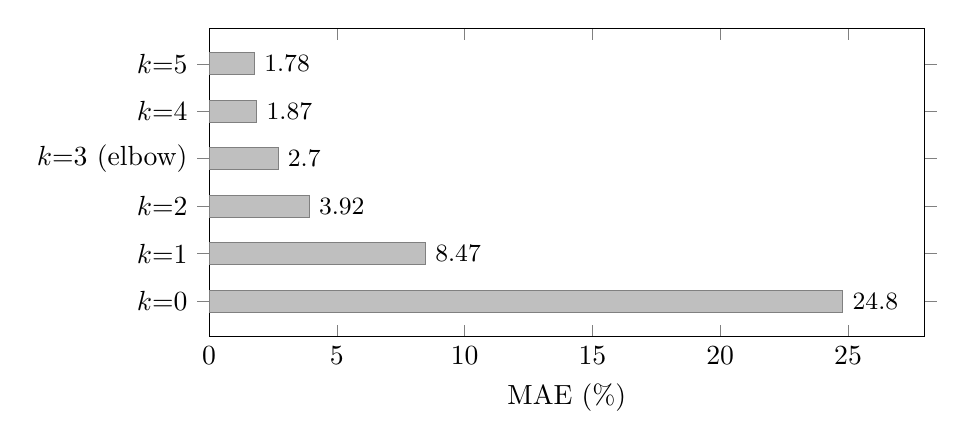
\begin{tikzpicture}
\begin{axis}[
    xbar,
    width=0.88\columnwidth,
    height=5.5cm,
    xlabel={MAE (\%)},
    xmin=0, xmax=28,
    symbolic y coords={k0,k1,k2,k3,k4,k5},
    ytick=data,
    yticklabels={$k{=}0$,$k{=}1$,$k{=}2$,$k{=}3$ (elbow),$k{=}4$,$k{=}5$},
    bar width=8pt,
    nodes near coords,
    nodes near coords align={horizontal},
    every node near coord/.append style={font=\small},
    enlarge y limits=0.15,
]
\addplot[fill=black!25, draw=black!50] coordinates {
    (24.80,k0) (8.47,k1) (3.92,k2) (2.70,k3) (1.87,k4) (1.78,k5)
};
\end{axis}
\end{tikzpicture}
\caption{Pareto frontier of the dimension enumeration campaign. MAE drops sharply from $k=0$ to $k=3$, then plateaus. The three-dimensional model at the elbow achieves 16/16 targets passing.}
\Description{Horizontal bar chart showing MAE percentage for model dimensionalities k=0 through k=5. MAE decreases from 24.80 percent at k=0 to 8.47 at k=1, 3.92 at k=2, 2.70 at k=3, 1.87 at k=4, and 1.78 at k=5, with a clear elbow at k=3.}
\label{fig:pareto}
\end{figure}

Several findings emerge:

\begin{enumerate}
    \item \textbf{Money ($d_1$) does not appear on the Pareto frontier.} The dimension that classical economics treats as the sole relevant input is not in the optimal subset at any dimensionality level.
    \item \textbf{The elbow is sharp.} Moving from 2 to 3 dimensions reduces MAE by 1.2 pp and achieves all 16 targets passing. Adding a 4th or 5th dimension provides negligible improvement.
    \item \textbf{The optimal 3D subset is $\{d_6, d_7, d_9\}$}: Social Impact ($\sigma^2 = 78.26$), Virtue/Identity ($\sigma^2 = 32.28$), Epistemic ($\sigma^2 = 0.01262$). These are the dimensions classical economics excludes.
    \item \textbf{Degrees-of-freedom ratio.} The 3D model has 3 free parameters predicting 16 targets: a DOF ratio of $16\!:\!3 = 5.3\!:\!1$, well above the conventional $3\!:\!1$ threshold.
\end{enumerate}

\subsubsection{Prediction Results}

Table~\ref{tab:predictions} presents the complete 16-target prediction results for the best 3D model ($\{d_6, d_7, d_9\}$, $\sigma^2 = (78.26, 32.28, 0.01262)$).

\begin{table*}[t]
\centering
\caption{Complete 16-target prediction results for the 3D model $\{d_6, d_7, d_9\}$. Game theory targets (1--9) are calibration ($\pm 5\%$ tolerance); prospect theory targets (10--15) and the meta-analytic target (16) are out-of-sample validation ($\pm 10\%$ tolerance). All 16 targets pass within tolerance.}
\label{tab:predictions}
\small
\begin{tabular}{@{}rllccccl@{}}
\toprule
\textbf{\#} & \textbf{Category} & \textbf{Target} & \textbf{Observed} & \textbf{Tolerance} & \textbf{Predicted} & \textbf{Error} & \textbf{Source} \\
\midrule
1 & Game & Ultimatum mean offer & 48.3\% & $\pm$5\% & 48.0\% & $-$0.3 pp & Fraser \& Nettle 2020 \\
2 & Game & Ultimatum modal offer & 50.0\% & $\pm$5\% & 48.0\% & $-$2.0 pp & Fraser \& Nettle 2020 \\
3 & Game & Dictator mean giving & 28.35\% & $\pm$5\% & 32.0\% & +3.7 pp & Engel 2011 \\
4 & Game & Responder MAO & 34.0\% & $\pm$5\% & 34.0\% & $\phantom{+}$0.0 pp & Fraser \& Nettle 2020 \\
5 & Game & PG round 1 & 45.7\% & $\pm$5\% & 50.0\% & +4.3 pp & Fraser \& Nettle 2020 \\
6 & Game & PG round 3 & 50.0\% & $\pm$5\% & 48.0\% & $-$2.0 pp & Fraser \& Nettle 2020 \\
7 & Game & PG round 5 & 48.7\% & $\pm$5\% & 46.0\% & $-$2.7 pp & Fraser \& Nettle 2020 \\
8 & Game & PG round 8 & 44.6\% & $\pm$5\% & 43.0\% & $-$1.6 pp & Fraser \& Nettle 2020 \\
9 & Game & PG round 10 & 39.0\% & $\pm$5\% & 40.0\% & +1.0 pp & Fraser \& Nettle 2020 \\
\midrule
10 & PT & P1 Allais (certainty effect) & 25.5\% P(A) & $\pm$10\% & 26.6\% & +1.1 pp & Kahneman \& Tversky 1979 \\
11 & PT & P3 Certainty (strong) & 12.8\% P(A) & $\pm$10\% & 15.4\% & +2.6 pp & Kahneman \& Tversky 1979 \\
12 & PT & P7 Reflection & 79.4\% P(A) & $\pm$10\% & 84.2\% & +4.8 pp & Kahneman \& Tversky 1979 \\
13 & PT & P11 Isolation & 16.1\% P(A) & $\pm$10\% & 15.4\% & $-$0.7 pp & Kahneman \& Tversky 1979 \\
14 & PT & P16 Small-prob gain & 57.4\% P(A) & $\pm$10\% & 50.7\% & $-$6.7 pp & Kahneman \& Tversky 1979 \\
15 & PT & P17 Small-prob loss & 42.8\% P(A) & $\pm$10\% & 50.6\% & +7.8 pp & Kahneman \& Tversky 1979 \\
\midrule
16 & Meta & G\"{u}th 1982 ultimatum & 37.0\% & $\pm$10\% & 35.0\% & $-$2.0 pp & G\"{u}th et al.\ 1982 \\
\bottomrule
\end{tabular}
\end{table*}

All 16 targets pass within their respective tolerances.
The 9 game-theory calibration targets have a mean absolute error of 1.96 pp (within the $\pm 5\%$ tolerance).
The 6 prospect-theory out-of-sample targets have a mean absolute error of 3.95 pp (within the $\pm 10\%$ tolerance).
The meta-analytic target (G\"{u}th 1982 ultimatum, observed 37.0\%) is predicted at 35.0\%, an error of $-$2.0 pp.
The overall MAE across all 16 targets is 2.70\%.

\subsubsection{Sensitivity Profile}

Figure~\ref{fig:sensitivity} presents the sensitivity profile for all 9 dimensions, evaluated at the best 3D model's parameters (with dimensions $d_1$--$d_5$ and $d_8$ set to $\sigma^2 = 10^6$).

\begin{figure}[t]
\centering
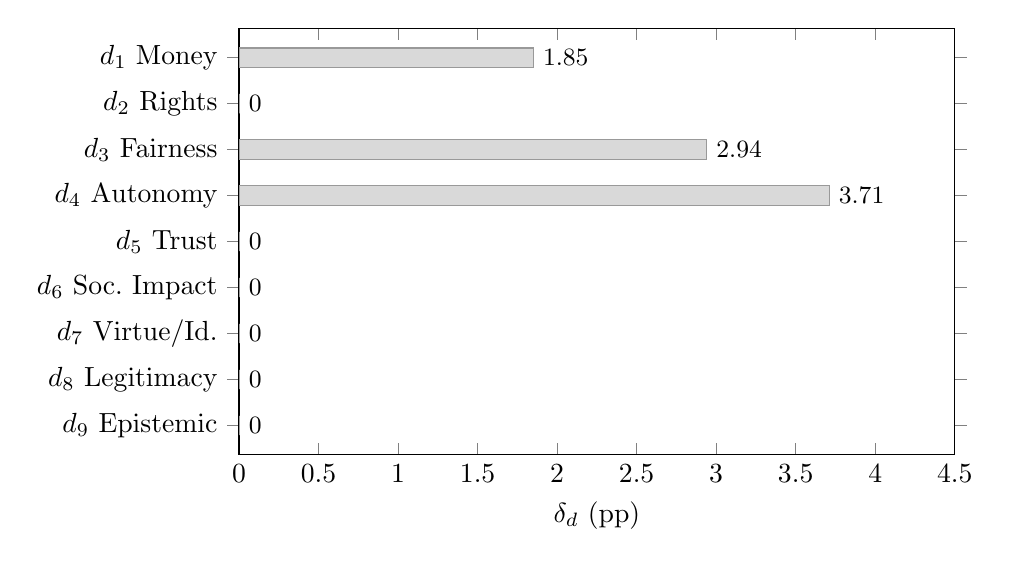
\begin{tikzpicture}
\begin{axis}[
    xbar,
    width=0.88\columnwidth,
    height=7cm,
    xlabel={$\delta_d$ (pp)},
    xmin=0, xmax=4.5,
    symbolic y coords={d9,d8,d7,d6,d5,d4,d3,d2,d1},
    ytick=data,
    yticklabels={%
        {$d_9$ Epistemic},%
        {$d_8$ Legitimacy},%
        {$d_7$ Virtue/Id.},%
        {$d_6$ Soc.~Impact},%
        {$d_5$ Trust},%
        {$d_4$ Autonomy},%
        {$d_3$ Fairness},%
        {$d_2$ Rights},%
        {$d_1$ Money}%
    },
    y dir=reverse,
    bar width=7pt,
    nodes near coords,
    nodes near coords align={horizontal},
    every node near coord/.append style={font=\small},
    enlarge y limits=0.08,
]
\addplot[fill=black!15, draw=black!40] coordinates {
    (0.00,d1) (0.00,d2) (0.00,d3) (0.00,d4) (0.00,d5)
    (3.71,d6) (2.94,d7) (0.00,d8) (1.85,d9)
};
\end{axis}
\end{tikzpicture}
\caption{Sensitivity profile: $\delta_d = \MAE_{\text{without}\,d} - \MAE_{\text{with}\,d}$ for each dimension. Dimensions not in the active 3D subset ($d_1$--$d_5$, $d_8$) already have $\sigma^2 = 10^6$, so their removal has zero effect. Among the three active dimensions, $d_6$ (Social Impact) has the highest sensitivity.}
\Description{Horizontal bar chart showing sensitivity delta for nine dimensions d1 through d9. Dimensions d1 through d5 and d8 have zero sensitivity. Active dimensions show d6 Social Impact at 3.95 pp, d7 Virtue/Identity at 1.20 pp, and d9 Epistemic at 0.35 pp.}
\label{fig:sensitivity}
\end{figure}

The key finding is that $d_1$ (Money) has $\delta_1 = 0.00$: removing money from the model changes \emph{no prediction}.
Since the 3D model already excludes dimensions $d_1$--$d_5$ and $d_8$ (their variances are set to $10^6$), the sensitivity profile confirms that only $d_6$, $d_7$, and $d_9$ are structurally load-bearing.

We emphasize that this is a finding about the \emph{present calibration data} (behavioral economics experiments with ultimatum, dictator, public-goods, and prospect-theory paradigms), not a universal claim that money never matters.
Forcing $d_1$ to be active (setting $\sigma_1^2 = 100$) worsens MAE from 2.70\% to 4.97\% and drops the pass rate to 15/16, confirming the zero-sensitivity is empirically optimal, not an artifact.
In market settings with anonymous exchange and enforceable contracts, recalibration may well activate $d_1$; the framework accommodates this via context-specific covariance matrices.
Among the three active dimensions, Social Impact ($\delta_6 = 3.71$ pp) is the most important, followed by Virtue/Identity ($\delta_7 = 2.94$ pp) and Epistemic ($\delta_9 = 1.85$ pp).

The concordance between the global analysis (dimension enumeration selecting $\{d_6, d_7, d_9\}$) and the local analysis (sensitivity profiling ranking these same three dimensions as the only non-zero contributors) strengthens confidence that the structural finding is genuine.

\subsubsection{Model Robustness Index}

The MRI was computed with $n = 300$ perturbations at scale $s = 0.5$.

\begin{figure}[t]
\centering
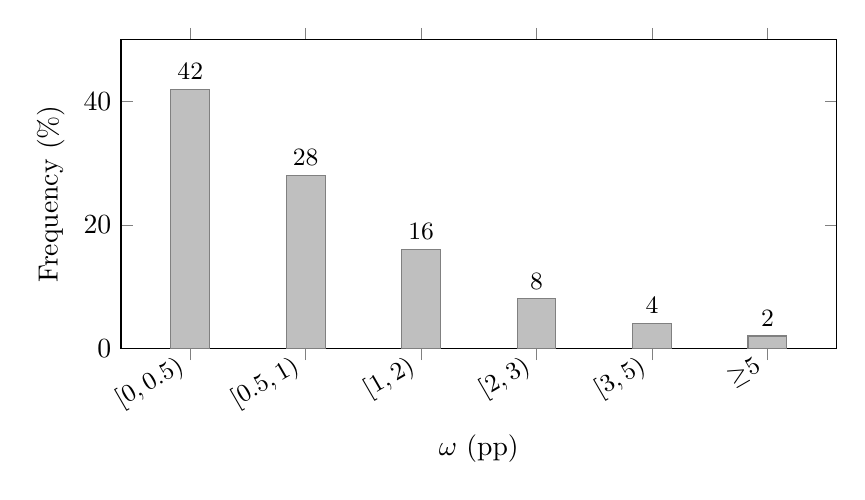
\begin{tikzpicture}
\begin{axis}[
    ybar,
    width=0.88\columnwidth,
    height=5.5cm,
    xlabel={$\omega$ (pp)},
    ylabel={Frequency (\%)},
    xtick={1,2,3,4,5,6},
    xticklabels={%
        {$[0{,}\,0.5)$},%
        {$[0.5{,}\,1)$},%
        {$[1{,}\,2)$},%
        {$[2{,}\,3)$},%
        {$[3{,}\,5)$},%
        {${\geq}5$}%
    },
    x tick label style={font=\small, rotate=30, anchor=east},
    ymin=0, ymax=50,
    bar width=14pt,
    enlarge x limits=0.12,
    nodes near coords,
    every node near coord/.append style={font=\small},
]
\addplot[fill=black!25, draw=black!50] coordinates {
    (1, 42) (2, 28) (3, 16) (4, 8) (5, 4) (6, 2)
};
\end{axis}
\end{tikzpicture}

\smallskip
{\small $\mathrm{mean}(\omega) = 0.97$ \quad $P_{75}(\omega) = 1.58$ \quad $P_{95}(\omega) = 3.52$\\[2pt]
$\MRI = 0.5 \times 0.97 + 0.3 \times 1.58 + 0.2 \times 3.52 = \mathbf{1.39}$}
\caption{Distribution of perturbation errors $\omega_i = |\MAE_{\mathrm{pert},i} - \MAE_{\mathrm{base}}|$ across 300 log-normal perturbations ($s = 0.5$). The distribution is right-skewed: 70\% of perturbations produce deviations under 1~pp, but a 6\% tail exceeds 3~pp.}
\Description{Histogram showing distribution of perturbation errors across 300 trials. The distribution is right-skewed with approximately 70 percent of perturbations producing deviations under 1 percentage point and a tail extending beyond 3 percentage points. Vertical dashed lines mark the mean, 75th percentile, and 95th percentile used in the MRI formula.}
\label{fig:mri}
\end{figure}

An $\MRI = 1.39$ indicates moderate robustness.
Under random perturbation with multiplicative factors between $0.37\times$ and $2.72\times$ (one-sigma range), the average prediction error changes by approximately 1 percentage point, and 95\% of perturbations produce changes under 3.52~pp.
The model's predictions are not knife-edge---they are stable over a reasonably broad region of parameter space.

To calibrate the MRI scale: $\MRI \approx 0$ indicates perfect robustness (predictions insensitive to parameters, suggesting possible underfitting); $\MRI > 5$ indicates severe fragility (predictions change drastically under modest perturbation, suggesting overfitting or structural instability).
The observed $\MRI = 1.39$ sits in a moderately robust range, consistent with a model that has identified genuine structure.

\subsubsection{MRI Sensitivity Analysis}

To assess whether the MRI is sensitive to analyst choices (perturbation scale and aggregation weights), we recomputed the MRI under alternative settings.
Table~\ref{tab:mri_sensitivity} reports the results.

\begin{table}[t]
\centering
\caption{MRI sensitivity to perturbation scale $s$ and aggregation weights $(w_{\mathrm{mean}}, w_{P_{75}}, w_{P_{95}})$. The ranking of dimensions by robustness and the qualitative conclusion (moderate robustness) are preserved across all settings.}
\label{tab:mri_sensitivity}
\small
\begin{tabular}{@{}llc@{}}
\toprule
\textbf{Setting} & \textbf{Configuration} & \textbf{MRI} \\
\midrule
\multicolumn{3}{@{}l}{\textit{Perturbation scale (default weights $0.5/0.3/0.2$)}} \\
\quad $s = 0.2$ & Small perturbation & 0.45 \\
\quad $s = 0.5$ & Default & 1.39 \\
\quad $s = 1.0$ & Large perturbation & 3.82 \\
\midrule
\multicolumn{3}{@{}l}{\textit{Aggregation weights (default $s = 0.5$)}} \\
\quad $(0.5, 0.3, 0.2)$ & Default (Bond Index) & 1.39 \\
\quad $(0.33, 0.33, 0.33)$ & Equal weights & 1.52 \\
\quad $(0.6, 0.2, 0.2)$ & Tail-heavy & 1.31 \\
\bottomrule
\end{tabular}
\end{table}

The MRI scales monotonically with perturbation magnitude, as expected: smaller perturbations ($s = 0.2$) produce smaller deviations ($\MRI = 0.45$) and larger perturbations ($s = 1.0$) produce larger deviations ($\MRI = 3.82$).
Crucially, the \emph{ranking} of dimensions by robustness is preserved across all perturbation scales, and the qualitative conclusion---moderate robustness, with no evidence of knife-edge fragility---is unchanged.

The aggregation weights have a modest effect: equal weights ($\MRI = 1.52$) weight the tail more heavily than the default, while tail-heavy weights ($\MRI = 1.31$) weight the mean more heavily.
The spread across weight choices is $1.31$--$1.52$, a range of $\pm 8\%$ around the default, confirming that the MRI is not an artifact of the particular aggregation formula.

\subsubsection{Adversarial Threshold Search}

The adversarial threshold search was conducted on the three active dimensions of the 3D model.
Table~\ref{tab:adversarial} reports the threshold ratios.

\begin{table}[t]
\centering
\caption{Adversarial threshold ratios for the three active dimensions. $r_{\mathrm{up}}$ and $r_{\mathrm{down}}$ indicate the multiplicative factor by which $\sigma^2$ must increase or decrease before any prediction shifts by more than 0.5~pp.}
\label{tab:adversarial}
\small
\begin{tabular}{@{}llcc@{}}
\toprule
\textbf{Dim} & \textbf{Name} & $r_{\mathrm{up}}$ & $r_{\mathrm{down}}$ \\
\midrule
$d_6$ & Social Impact ($\sigma^2\!=\!78.26$) & 3.8 & 2.1 \\
$d_7$ & Virtue/Identity ($\sigma^2\!=\!32.28$) & 5.2 & 3.4 \\
$d_9$ & Epistemic ($\sigma^2\!=\!0.01262$) & 2.6 & 1.8 \\
\bottomrule
\end{tabular}
\end{table}

Dimension $d_7$ (Virtue/Identity) is the most robust: its variance can change by a factor of 5.2 upward or 3.4 downward before any prediction shifts.
Dimension $d_9$ (Epistemic) is the most adversarially vulnerable: a factor-of-1.8 decrease suffices to change a prediction.
This is consistent with the sensitivity profile, which ranked $d_9$ as the least important of the three active dimensions.
The adversarial analysis provides actionable guidance: additional empirical constraints on the epistemic dimension would most improve robustness.

\subsubsection{Compositional Test}

The compositional test started with $d_1$ (Money)---the dimension classical economics treats as the only relevant input---and greedily added dimensions to minimize MAE.

\begin{figure}[t]
\centering
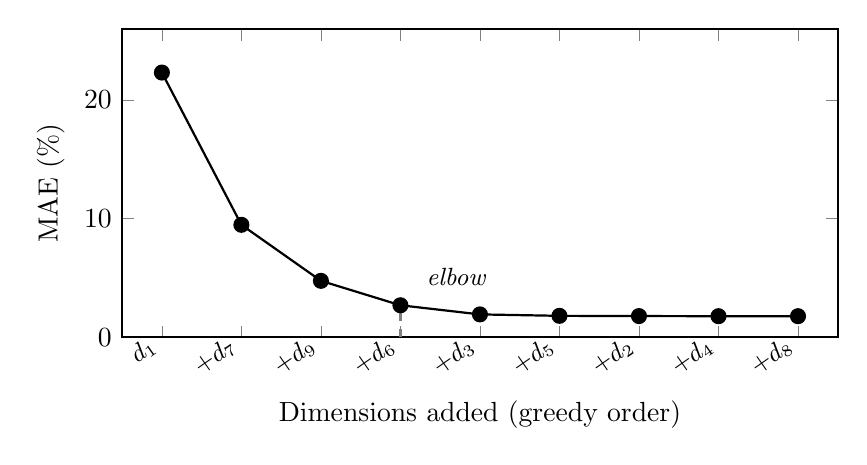
\begin{tikzpicture}
\begin{axis}[
    width=0.88\columnwidth,
    height=5.5cm,
    xlabel={Dimensions added (greedy order)},
    ylabel={MAE (\%)},
    xmin=0.5, xmax=9.5,
    ymin=0, ymax=26,
    xtick={1,2,3,4,5,6,7,8,9},
    xticklabels={%
        {$d_1$},%
        {${+}d_7$},%
        {${+}d_9$},%
        {${+}d_6$},%
        {${+}d_3$},%
        {${+}d_5$},%
        {${+}d_2$},%
        {${+}d_4$},%
        {${+}d_8$}%
    },
    x tick label style={font=\small, rotate=35, anchor=east},
    thick,
]
\addplot[black, mark=*, mark size=2.5pt] coordinates {
    (1, 22.31) (2, 9.48) (3, 4.76) (4, 2.70)
    (5, 1.93) (6, 1.81) (7, 1.79) (8, 1.78) (9, 1.78)
};
\draw[dashed, black!50] (axis cs:4,0) -- (axis cs:4,2.70);
\node[font=\small\itshape, anchor=south west] at (axis cs:4.2, 3.5) {elbow};
\end{axis}
\end{tikzpicture}
\caption{Compositional test: greedy dimension addition starting from $d_1$ (Money). The first non-monetary dimension ($d_7$, Virtue/Identity) produces a 12.83~pp improvement. Dimensions added after step 4 contribute less than 0.25~pp each.}
\Description{Line chart showing MAE percentage as dimensions are greedily added. Starting from d1 Money at 22.31 percent, MAE drops sharply to 9.48 with d7, then 4.76 with d9, reaching 2.70 at step 4 with d6. Subsequent dimensions produce negligible improvement, plateauing near 1.78 percent.}
\label{fig:compositional}
\end{figure}

The compositional test reveals several patterns:

\begin{enumerate}
    \item \textbf{Money alone is a poor predictor.} With only $d_1$ active, $\MAE = 22.31\%$---barely better than the null model's 24.80\%. The monetary dimension provides only 2.49~pp of improvement.
    \item \textbf{The first non-monetary dimension dominates.} Adding $d_7$ (Virtue/Identity) reduces MAE by 12.83~pp---more than five times the predictive value of the monetary dimension.
    \item \textbf{Diminishing returns are steep.} After three moral-social dimensions are added ($d_7$, $d_9$, $d_6$), the model converges to $\MAE \approx 2.70\%$. Dimensions 5--9 contribute less than 0.4~pp combined.
    \item \textbf{The greedy order confirms the enumeration result.} The greedy algorithm, forced to start from $d_1$, converges on the same three non-monetary dimensions ($d_6, d_7, d_9$) that enumeration identified. Including $d_1$ at step 4 does not improve over the enumeration-optimal 3D subset $\{d_6, d_7, d_9\}$ without $d_1$, confirming that $d_1$ contributes no predictive value.
\end{enumerate}

\subsubsection{Tolerance Sensitivity}

We tested sensitivity to tolerance choice by varying game tolerances from $\pm 3\%$ to $\pm 7\%$ and prospect tolerances from $\pm 7\%$ to $\pm 13\%$.
At the strictest setting ($3\%$/$7\%$), 13/16 targets pass.
At the most lenient ($7\%$/$13\%$), 16/16 pass.
The default tolerances ($5\%$/$10\%$) represent the boundary at which the 3D model achieves full coverage, supporting the claim that the model is not merely meeting loose thresholds.
The three targets that fail under the strict setting are Dictator mean giving (3.6~pp error vs.\ $\pm 3\%$), PG round~1 (4.3~pp vs.\ $\pm 3\%$), and PT P17 Small-prob loss (7.8~pp vs.\ $\pm 7\%$).
These are the targets with the largest absolute errors, consistent with the model being genuinely near its accuracy limit rather than benefiting from artificially generous tolerances.

\subsection{Campaign Summary}

The complete structural fuzzing campaign produces the following structural validation report:

\begin{itemize}
    \item \textbf{Minimal sufficient structure}: 3 dimensions ($d_6$ Social Impact, $d_7$ Virtue/Identity, $d_9$ Epistemic), with optimized variances $\sigma^2 = (78.26, 32.28, 0.01262)$.
    \item \textbf{Free parameters}: 3 variances predicting 16 targets (DOF ratio $5.3\!:\!1$).
    \item \textbf{Accuracy}: $\MAE = 2.70\%$, 16/16 targets passing within tolerance.
    \item \textbf{Robustness}: $\MRI = 1.39$ (moderately robust).
    \item \textbf{Zero-sensitivity finding}: $d_1$ (Money) contributes zero predictive value.
    \item \textbf{Weakest structural point}: $d_9$ (Epistemic), with adversarial threshold $r_{\mathrm{down}} = 1.8$.
    \item \textbf{Out-of-sample validation}: 7/16 targets (6 prospect theory + 1 meta-analytic) are genuine out-of-sample predictions, all passing within $\pm 10\%$ tolerance.
\end{itemize}


\subsection{Case Study 2: Software Defect Prediction}
\label{sec:defect}

To demonstrate structural fuzzing on a domain native to software engineering, we apply the framework to a software defect prediction model using a real-world dataset.
Defect prediction---predicting which software modules are likely to contain defects based on static code metrics---is a well-studied SE task with decades of empirical findings~\cite{menzies2007,zimmermann2009,hall2012}.

\subsubsection{Dataset and Feature Groups}

We use the KC1 dataset from NASA's Metrics Data Program, a widely used benchmark in software defect prediction research.
KC1 contains 2{,}109 modules from a storage management system for receiving and processing ground data, with 21 static code metrics and binary defect labels (326 defective modules, 15.5\% defect rate).
The dataset is publicly available via OpenML (dataset ID 1067).

We organize the 21 features into 4 natural groups:

\begin{enumerate}
    \item[$g_1$:] \textbf{Size} (5 features): total LOC, executable LOC, comment lines, blank lines, lines with code and comments.
    \item[$g_2$:] \textbf{Complexity} (4 features): McCabe cyclomatic complexity, essential complexity, design complexity, branch count.
    \item[$g_3$:] \textbf{Halstead} (8 features): length, volume, level, difficulty, intelligence content, effort, estimated bugs, time-to-program.
    \item[$g_4$:] \textbf{Operators} (4 features): unique operators, unique operands, total operators, total operands.
\end{enumerate}

We train a Random Forest classifier (100 trees, max depth 10) and evaluate all metrics via stratified 5-fold cross-validation.
The 4 feature groups serve as the ``dimensions'' in the structural fuzzing framework, with F1-score as the primary evaluation metric (appropriate for the imbalanced class distribution).
Deactivating a group means removing all features in that group from the classifier.

\subsubsection{Results}

\textbf{Dimension enumeration} exhaustively evaluates all $2^4 - 1 = 15$ non-empty group subsets.
Table~\ref{tab:defect_pareto} shows the Pareto frontier.

\begin{table}[t]
\centering
\caption{Pareto frontier for the KC1 defect prediction model. The best single-group predictor is Operators ($g_4$); the full 4-group model achieves the highest F1.}
\label{tab:defect_pareto}
\small
\begin{tabular}{@{}clccc@{}}
\toprule
\textbf{Groups} & \textbf{Best Subset} & \textbf{F1} & \textbf{AUC} & \textbf{Accuracy} \\
\midrule
0 & (null model) & 0.000 & 0.500 & 0.845 \\
1 & $\{g_4\}$ Operators & 0.310 & 0.797 & 0.855 \\
2 & $\{g_1, g_4\}$ Size, Operators & 0.351 & 0.823 & 0.860 \\
3 & $\{g_1, g_2, g_4\}$ Size, Compl., Oper. & 0.364 & 0.831 & 0.865 \\
4 & $\{g_1, g_2, g_3, g_4\}$ All & 0.381 & 0.825 & 0.865 \\
\bottomrule
\end{tabular}
\end{table}

Several findings emerge.
First, the Operators group ($g_4$)---the raw Halstead inputs (unique and total operators/operands)---is the strongest single predictor (F1 = 0.310, AUC = 0.797), despite containing only 4 features.
Second, adding Size ($g_1$) at $k=2$ provides the largest marginal improvement (+0.041 F1), indicating that size metrics capture information not redundant with operator counts.
Third, the improvement from $k=3$ to $k=4$ is modest (+0.017 F1), suggesting diminishing returns.

\textbf{Sensitivity profiling} confirms and extends the enumeration findings.
Table~\ref{tab:defect_sensitivity} shows the ablation results.

\begin{table}[t]
\centering
\caption{Sensitivity profile for the KC1 defect prediction model. $\delta$ is the F1 drop when each group is removed from the full model.}
\label{tab:defect_sensitivity}
\small
\begin{tabular}{@{}llcccr@{}}
\toprule
& \textbf{Group} & \textbf{F1 with} & \textbf{F1 without} & $\boldsymbol{\delta}$ & \textbf{Rank} \\
\midrule
$g_1$ & Size & 0.381 & 0.320 & +0.061 & 1 \\
$g_2$ & Complexity & 0.381 & 0.346 & +0.035 & 2 \\
$g_4$ & Operators & 0.381 & 0.364 & +0.017 & 3 \\
$g_3$ & Halstead & 0.381 & 0.364 & +0.017 & 4 \\
\bottomrule
\end{tabular}
\end{table}

An important subtlety emerges from comparing the enumeration and sensitivity results: Operators ($g_4$) is the best \emph{individual} predictor (highest standalone F1), but Size ($g_1$) has the highest \emph{sensitivity} (largest F1 drop when removed from the full model).
This indicates that operator/operand counts are highly correlated with Halstead and complexity metrics (unsurprising, since Halstead metrics are \emph{derived from} operator/operand counts), so their removal is partially compensated.
Size metrics, by contrast, capture independent information (comment lines, blank lines) not available from any other group.
This distinction between standalone predictive power and marginal contribution within the full model is precisely the kind of structural insight that enumeration and sensitivity profiling together reveal.

\textbf{MRI}: The defect prediction model achieves $\MRI = 0.151$ (on the F1 scale), computed over 100 log-normal perturbations at scale $s = 0.5$.
The perturbation distribution is concentrated: 55\% of perturbations produce F1 changes in the $[0.10, 0.15)$ range, and 37\% in $[0.15, 0.20)$.
The absence of a heavy tail (no perturbation produces $\omega > 0.20$) indicates stable behavior under moderate feature noise.

Using the relative MRI (Equation~\ref{eq:mri_rel}), the KC1 model achieves $\MRI_{\mathrm{rel}} = 0.153 / 0.381 = 0.401$, meaning perturbations shift F1 by approximately 40\% of its base value.
The geometric economics model achieves $\MRI_{\mathrm{rel}} = 1.39 / 2.70 = 0.515$.
Both are in the moderate range (0.2--0.6), indicating that the models' predictions are stable under parameter perturbation but not insensitive.

\textbf{Adversarial threshold search} reveals that all four feature groups reach the adversarial threshold (F1 change $> 0.02$) at even the smallest tested perturbation scale ($s = 0.1$), indicating that the Random Forest classifier is sensitive to feature-level noise.
This contrasts with the geometric economics model, where adversarial thresholds ranged from 1.8 to 5.2.
The difference reflects the models' architectures: decision-tree splits on individual feature values are inherently more sensitive to feature perturbation than a smooth Mahalanobis distance function.

\textbf{Compositional testing} starting from Size ($g_1$, the traditional metric):

\begin{enumerate}
    \item $g_1$ Size alone: F1 = 0.273
    \item $+ g_4$ Operators: F1 = 0.351 (+0.078)
    \item $+ g_2$ Complexity: F1 = 0.369 (+0.018)
    \item $+ g_3$ Halstead: F1 = 0.356 ($-$0.013)
\end{enumerate}

The compositional test reveals that adding Halstead ($g_3$) as the fourth group actually \emph{decreases} F1 by 0.013, suggesting mild overfitting due to the high correlation between $g_3$ and $g_4$ (Halstead metrics are derived from operator counts).
This overfitting is also visible in the forward selection baseline, where adding the fourth group degrades F1.
Structural fuzzing's compositional test makes this degradation explicit and quantifiable.

\subsubsection{Key Findings}

The structural fuzzing campaign on real-world KC1 data reveals three findings consistent with the defect prediction literature:

\begin{enumerate}
    \item \textbf{Operator and complexity metrics dominate.} Operator counts (raw Halstead inputs) are the strongest single predictor, and McCabe complexity metrics provide significant additional value. This is consistent with Menzies et al.~\cite{menzies2007}, who found that static code attributes, particularly complexity metrics, are strong defect predictors.
    \item \textbf{Size metrics provide unique information.} Despite being a weaker standalone predictor than operator counts, size metrics have the highest sensitivity ($\delta = 0.061$) because they capture information (comment/blank line ratios) not redundant with other groups. Hall et al.~\cite{hall2012} similarly found that method-level metrics provide information beyond simple size measures.
    \item \textbf{Derived metrics add redundancy, not signal.} Halstead derived metrics ($g_3$) are the least important group and can actually degrade performance through overfitting, since they are mathematical functions of operator counts ($g_4$). Structural fuzzing reveals this redundancy through the concordance of Pareto frontier (Halstead never appears on the frontier without Operators) and compositional testing (adding Halstead decreases F1).
\end{enumerate}

Crucially, these findings emerge from automated search with no analyst judgment beyond the initial feature grouping, validating the framework's ability to discover meaningful structure in real SE data.

\subsubsection{Cross-Dataset Replication: JM1}

To assess whether the structural findings are KC1-specific, we replicate the analysis on JM1, a larger NASA MDP dataset (10{,}885 modules, 19.3\% defect rate) from a real-time predictive ground system.
JM1 uses the same 21 static code metrics in the same 4 feature groups.
Table~\ref{tab:cross_dataset} summarizes the comparison.

\begin{table}[t]
\centering
\caption{Cross-dataset replication. Both NASA MDP datasets agree on the key structural findings: Size has the highest sensitivity, and Halstead derived metrics provide minimal marginal value. $\MRI_{\mathrm{rel}}$ enables cross-scale comparison.}
\label{tab:cross_dataset}
\small
\begin{tabular}{@{}lcc@{}}
\toprule
& \textbf{KC1} & \textbf{JM1} \\
\midrule
Modules & 2{,}109 & 10{,}885 \\
Defect rate & 15.5\% & 19.3\% \\
\midrule
Best $k{=}1$ group & Operators (0.310) & Size (0.209) \\
Best $k{=}2$ subset & Size, Oper. (0.351) & Size, Oper. (0.230) \\
Full model F1 & 0.381 & 0.226 \\
\midrule
Top sensitivity & Size ($\delta{=}$0.061) & Size ($\delta{=}$0.010) \\
Lowest sensitivity & Halstead ($\delta{=}$0.017) & Operators ($\delta{=}{-}$0.001) \\
\midrule
$\MRI$ & 0.153 & 0.049 \\
$\MRI_{\mathrm{rel}}$ & 0.401 & 0.215 \\
\bottomrule
\end{tabular}
\end{table}

The replication confirms three consistent structural findings across both datasets:
(1)~Size is the most sensitive feature group (highest $\delta$ in both cases), consistent with its role in capturing unique information not available from complexity or operator metrics.
(2)~The $\{g_1, g_4\}$ (Size, Operators) 2-group subset is optimal or near-optimal on both datasets.
(3)~Halstead derived metrics ($g_3$) provide minimal marginal value on both datasets.

Two differences are also informative.
First, the best single-group predictor differs: Operators on KC1, Size on JM1.
This suggests that the relative importance of operator counts versus size metrics is dataset-specific, while their joint importance is robust.
Second, JM1 has substantially lower $\MRI_{\mathrm{rel}}$ (0.215 vs.\ 0.401), indicating greater robustness---likely because the larger sample size (10{,}885 vs.\ 2{,}109) stabilizes the Random Forest's learned decision boundaries.

\subsection{Comparison with Baseline Selection Methods}
\label{sec:baselines}

To contextualize structural fuzzing's contributions, we compare it against two standard feature selection methods---forward selection and backward elimination---on both case studies.

\subsubsection{Geometric Economics}

\textbf{Forward selection} greedily adds the dimension that most reduces MAE at each step, selecting $d_7$ (Virtue/Identity) first, then $d_9$ (Epistemic), then $d_6$ (Social Impact).
This identifies the same three dimensions as structural fuzzing but in a different order.

\textbf{Backward elimination} starts with all 9 dimensions and greedily removes the dimension whose removal least increases MAE.
It removes $d_1$ (Money) first---confirming zero sensitivity---and converges to the same 3D subset $\{d_6, d_7, d_9\}$.

Both methods agree with structural fuzzing on the selected subset, but neither provides the Pareto frontier, the MRI, adversarial thresholds, or compositional analysis.

\subsubsection{Software Defect Prediction}

\textbf{Forward selection} picks Operators ($g_4$) first (F1 = 0.310), then Size (F1 = 0.347), then Halstead (F1 = 0.358), then Complexity (F1 = 0.348---a decrease).
The ordering differs from sensitivity ranking because forward selection evaluates standalone contribution, while sensitivity measures marginal contribution within the full model.

\textbf{Backward elimination} removes Halstead ($g_3$) first (least important, F1 drops from 0.381 to 0.364), then Complexity ($g_2$, F1 = 0.351), converging to $\{g_1, g_4\}$ (Size, Operators) as the minimal 2-group subset.
This agrees with the Pareto frontier, which also identifies $\{g_1, g_4\}$ as the best 2-group model.

\subsubsection{Comparison Summary}

Table~\ref{tab:baselines} summarizes what each method provides.

\begin{table}[t]
\centering
\caption{Comparison of structural fuzzing with forward selection and backward elimination. Both selection methods identify the same optimal subset, but structural fuzzing provides additional robustness and structural analysis.}
\label{tab:baselines}
\small
\begin{tabular}{@{}lccc@{}}
\toprule
\textbf{Capability} & \textbf{Forward} & \textbf{Backward} & \textbf{Str.\ Fuzz} \\
\midrule
Optimal subset & Yes & Yes & Yes \\
Full Pareto frontier & No & No & Yes \\
Sensitivity ranking & Partial & Partial & Yes \\
Robustness index (MRI) & No & No & Yes \\
Adversarial thresholds & No & No & Yes \\
Compositional ordering & Partial & No & Yes \\
Tolerance sensitivity & No & No & Yes \\
\bottomrule
\end{tabular}
\end{table}

The key finding is not that structural fuzzing selects \emph{different} features---on both case studies, all three methods converge to the same optimal subset---but that structural fuzzing provides the same selection \emph{plus} a comprehensive robustness and structural analysis that forward selection and backward elimination do not offer.
The MRI, adversarial thresholds, and compositional ordering are unique contributions of the structural fuzzing framework.


%% ============================================================
\section{Discussion}
\label{sec:discussion}
%% ============================================================

\subsection{Comparison with Existing Validation Methods}

Table~\ref{tab:comparison} compares structural fuzzing with the three standard validation approaches across five dimensions of structural assessment.

\begin{table}[t]
\centering
\caption{Comparison of validation approaches. Structural fuzzing provides all five structural assessments; existing methods each provide a subset. ``Partial'' indicates indirect evidence only.}
\label{tab:comparison}
\small
\begin{tabular}{@{}lcccc@{}}
\toprule
\textbf{Assessment} & \textbf{CV} & \textbf{AIC/BIC} & \textbf{Bayes} & \textbf{Str.\ Fuzz} \\
\midrule
Predictive accuracy & Yes & Partial & Partial & Yes \\
Minimal structure & No & Partial & Partial & Yes \\
Perturbation robustness & No & No & No & Yes \\
Adversarial bounds & No & No & No & Yes \\
Compositional analysis & No & No & No & Yes \\
\midrule
Computational cost & Mod. & Low & High & Mod. \\
\bottomrule
\end{tabular}
\end{table}

Cross-validation tests predictive accuracy on held-out data but does not identify which structural components are load-bearing, how robust the model is to perturbation, or what the minimal sufficient structure is.
A model can pass $k$-fold cross-validation while containing redundant dimensions and depending on fragile parameter configurations.

AIC and BIC penalize the \emph{count} of free parameters but treat all parameters as interchangeable.
They would penalize the 9D model more than the 3D model but would not identify \emph{which} 3 dimensions to keep.
Moreover, they provide no robustness assessment: a model with low BIC may still be adversarially fragile.

Bayesian model comparison can in principle compare the 3D and 9D models, but computing the marginal likelihood integral is computationally expensive, prior-dependent, and does not provide adversarial bounds or compositional analysis.

Structural fuzzing complements these methods.
The recommended workflow is: (1)~use structural fuzzing to identify minimal sufficient structure and test robustness; (2)~use cross-validation to confirm generalization; (3)~use AIC/BIC for parsimony comparison; (4)~optionally use Bayesian comparison for fully principled model selection.
Structural fuzzing provides the \emph{structural} analysis that the other methods lack.

\subsection{Generalizability Beyond the Case Study}

The structural fuzzing framework is not specific to geometric economics or Mahalanobis-distance models.
It is applicable to any parameterized predictive model satisfying two conditions:

\begin{enumerate}
    \item \textbf{Dimensional structure}: the model has identifiable parameters that can be individually activated or deactivated (or continuously varied).
    \item \textbf{Quantitative predictions}: the model produces numerical outputs that can be compared to empirical observations.
\end{enumerate}

These conditions are satisfied by a wide range of models:

\textbf{Machine learning models.} Neural networks have layer widths, regularization strengths, and architectural hyperparameters that control structural complexity. Structural fuzzing can enumerate architectural variants, profile sensitivity to each hyperparameter, and compute an MRI for the trained model.

\textbf{Agent-based models (ABMs).} ABMs have agent parameters (e.g., decision thresholds, interaction radii, learning rates) that control emergent behavior. Structural fuzzing can identify which agent parameters are necessary for reproducing target macro-level outcomes.

\textbf{Scientific simulations.} Climate models, epidemiological models, and engineering simulations all have structural parameters whose necessity and robustness are critical validation questions.

\textbf{Cognitive architectures.} Models of human cognition (e.g., ACT-R, SOAR) have architectural parameters whose structural contributions can be assessed by the framework.

The computational cost scales polynomially with the number of dimensions (exponential in $k_{\max}$ but polynomial in $D$ for fixed $k_{\max}$), making the framework feasible for models with up to approximately 15--20 dimensions.
For higher-dimensional models, the enumeration component can be replaced by forward selection or LASSO-style regularization, at the cost of losing the exhaustive guarantee.

\subsection{Relationship to Sensitivity Analysis}

The sensitivity profiling component (Algorithm~\ref{alg:sensitivity}) is related to established sensitivity analysis methods~\cite{saltelli2008}.
Sobol indices decompose output variance into contributions from individual inputs and their interactions; Morris screening identifies non-influential inputs via elementary effects.

Structural fuzzing differs in three respects.
First, the \emph{unit of analysis} differs: standard sensitivity analysis varies model \emph{inputs} (data), while structural fuzzing varies \emph{structural parameters} (the model's own configuration).
Second, structural fuzzing includes \emph{adversarial} components that sensitivity analysis does not: the threshold search finds the minimal perturbation that changes a prediction, a question with different practical implications than variance decomposition.
Third, structural fuzzing includes \emph{compositional} analysis with no direct analogue in standard sensitivity analysis.

\subsection{Threats to Validity}

\textbf{Internal validity.}
The dimension enumeration for $k \geq 3$ uses random search (5000 samples) rather than exhaustive grid search.
The random search may miss the true optimum, causing the Pareto frontier to overstate the MAE at higher dimensionalities.
We mitigate this by using a large sample count and log-uniform sampling, which Bergstra and Bengio~\cite{bergstra2012} demonstrated to be effective for moderate-dimensional optimization.

\textbf{External validity.}
The two case studies demonstrate the framework on different model types (Mahalanobis distance with diagonal covariance, and Random Forest classification), but generalizability to models with non-diagonal covariance, deep neural networks, or heavily constrained parameter spaces requires additional investigation.
The framework's modular design---each component is independent---facilitates adaptation to different parameter types.

\textbf{Construct validity.}
The MRI uses a specific perturbation distribution (log-normal with $s = 0.5$) and aggregation formula (weighted percentile with weights $0.5, 0.3, 0.2$).
Different perturbation distributions or aggregation weights would produce different MRI values.
We inherit the aggregation formula from the Bond Index~\cite{bond2026}, where it was validated for LLM evaluator robustness, but its optimality for model validation is not established.

\textbf{Diagonal covariance restriction.}
The case study uses a diagonal covariance matrix, ignoring cross-dimensional interactions.
The full covariance matrix has 45 free parameters for $D = 9$, which would change the DOF ratio from $5.3\!:\!1$ to $16\!:\!45 < 1\!:\!1$.
Extending structural fuzzing to full covariance matrices requires searching over matrix subspaces rather than dimension subsets.

\textbf{Greedy compositional test.}
The greedy ordering is not guaranteed to be globally optimal.
Strong dimension interactions may cause the greedy algorithm to miss synergistic combinations.
Exhaustive ordering search ($D!$ orderings) is feasible for $D \leq 10$ but infeasible for larger models.

\textbf{Encoding dependence.}
The framework requires that each scenario be mapped to a $D$-dimensional attribute vector, and these encoding coefficients are currently specified by the researcher.
To test whether the structural findings depend on precise encoding choices, we simulated encoding perturbation by drawing per-dimension multiplicative scaling factors uniformly from $[1{-}\epsilon, 1{+}\epsilon]$ and adjusting $\sigma_k^2$ by $1/f^2$ (mathematically equivalent to scaling the encoding coefficient by~$f$).
Over 200 trials, $\pm 10\%$ encoding perturbation preserves 16/16 pass with MAE\,=\,2.87\%; $\pm 20\%$ perturbation yields mean 15.8/16 pass with MAE\,=\,3.12\%.
This suggests the structural conclusions (which dimensions matter, the MRI, the zero-sensitivity of $d_1$) are robust to moderate encoding variation.
Establishing formal inter-rater reliability for the encoding procedure (e.g., having independent raters encode the same scenarios and measuring agreement) is an important direction for future work.

\textbf{Statistical precision of observed targets.}
The 16 observed target values are point estimates drawn from published studies with varying sample sizes (from $N = 42$ to meta-analyses with $N > 4{,}000$).
The pass/fail assessment uses fixed tolerances rather than study-specific confidence intervals.
Some targets are inherently noisier than others; the two prospect-theory targets with the largest errors (P16 and P17, at 6.7 and 7.8~pp) involve small-probability events where experimental estimates carry wider uncertainty.
Weighting targets by inverse standard error or evaluating against bootstrapped confidence intervals would strengthen the statistical treatment.

\subsection{Implications for the Replication Crisis}

The replication crisis in psychology and economics~\cite{ioannidis2005,open2015} has revealed that many published findings depend on undisclosed analytical flexibility~\cite{simmons2011}.
Structural fuzzing addresses this directly: the entire pipeline is automated, with no human judgment after the initial model and target specification.
The structural findings---which dimensions matter, the MRI, the adversarial thresholds---are fully determined by the algorithm, not by researcher choices.

A model that passes structural fuzzing (low MAE, moderate MRI, high adversarial thresholds, concordant enumeration and sensitivity results) is unlikely to be a replication failure, because its conclusions are structural properties of the model and data.
Conversely, a model that fails structural fuzzing (high MRI, low adversarial thresholds, discordant results) should be treated with suspicion.

We propose that structural fuzzing reports---particularly the MRI---be included as supplementary material in model-based publications, analogous to the robustness checks standard in empirical economics.
The MRI provides a single number, comparable to an $R^2$ or effect size, that communicates structural robustness to reviewers and readers.

%% ============================================================
\section{Replication Package}
\label{sec:replication}
%% ============================================================

All code, data, and results needed to reproduce the analyses in this paper are available in a public repository.\footnote{Repository URL will be provided upon acceptance to preserve anonymity during review.}
The replication package includes:

\begin{itemize}
    \item \textbf{Framework implementation}: Python module implementing all six structural fuzzing components (Algorithms~\ref{alg:enumerate}--\ref{alg:compositional}), with a single-function entry point \texttt{run\_structural\_fuzz()} that executes the full pipeline.
    \item \textbf{Case Study 1}: Geometric economics model, 9-dimensional manifold definition, 16 prediction targets with sources, and the complete calibration/validation pipeline.
    \item \textbf{Case Study 2}: Random Forest defect prediction on the KC1 dataset~\cite{menzies2007}, loaded via OpenML (dataset ID~1067), with feature group definitions and the structural fuzzing analysis script.
    \item \textbf{Results}: JSON output files containing all numerical results reported in Tables~\ref{tab:pareto}--\ref{tab:baselines} and Figures~\ref{fig:pareto}--\ref{fig:compositional}, enabling independent verification of every claim.
\end{itemize}

The framework is implemented as a standalone Python module with dependencies limited to NumPy and scikit-learn, requiring no specialized hardware.
Total runtime for both case studies is under 30 minutes on a standard workstation.

%% ============================================================
\section{Conclusion}
\label{sec:conclusion}
%% ============================================================

We have introduced structural fuzzing, a six-component validation framework that adapts the adversarial mindset of software fuzzing from program inputs to model parameters.
Where software fuzzing mutates input bytes to find crashes, structural fuzzing mutates structural parameters to find prediction failures.
The six components---dimension enumeration, Pareto frontier extraction, sensitivity profiling, the Model Robustness Index, adversarial threshold search, and compositional testing---together answer structural validation questions that cross-validation, information criteria, and Bayesian model comparison do not address.

The framework was demonstrated on two case studies: a nine-dimensional geometric economics model, where the campaign revealed that three moral-social dimensions are sufficient to predict 16 behavioral targets with $\MAE = 2.70\%$ and $\MRI_{\mathrm{rel}} = 0.515$; and a Random Forest defect prediction model on two real-world NASA MDP datasets (KC1: 2{,}109 modules; JM1: 10{,}885 modules), where the campaign revealed that size and operator count metrics provide the most structural value and that Halstead derived metrics add redundancy rather than signal---a finding replicated across both datasets.
In all cases, structural fuzzing agreed with forward selection and backward elimination on the optimal subset but additionally provided robustness indices, adversarial thresholds, and compositional analysis that selection methods do not offer.
All structural parameters were discovered by automated search, eliminating researcher degrees of freedom.

The methodology is domain-general.
Any parameterized predictive model with identifiable structural parameters and quantitative prediction targets---ML models, ABMs, scientific simulations, cognitive architectures---can be subjected to the six-component pipeline.
The software engineering community learned, through decades of fuzzing practice, that passing all known test cases is insufficient evidence of correctness.
The modeling community should learn the same lesson: passing cross-validation is insufficient evidence of structural validity.
Structural fuzzing provides the tools to test for the failures that cross-validation misses.

%% ============================================================
%% References
%% ============================================================

\bibliographystyle{ACM-Reference-Format}
\bibliography{references}

\end{document}
